% /* cspell:disable */
\documentclass[a4paper,12pt]{book}

% import package
\usepackage{graphics}   % include graphics
\usepackage{float}      % h!

% figure
\usepackage{tikz}
\usepackage{pgfplots}
\usepackage{graphicx}
\usepackage{subcaption}

% page
\usepackage{fancyhdr}
\usepackage{setspace}
\usepackage{sectsty}

% math
\usepackage{amssymb}
\usepackage{amsmath}

% fancyhdr setting
\pagestyle{fancy}
\fancyhead{}
\fancyhead[LO]{\bfseries\rightmark}
\fancyhead[RO]{}
\fancyhead[RE]{\bfseries\leftmark}
\fancyhead[LE]{}

% page setting
\doublespacing
\allsectionsfont{\singlespacing}
\raggedbottom

% math symbols
\DeclareMathOperator*{\argmin}{arg\,min}
\DeclareMathOperator*{\argmax}{arg\,max}
\newcommand*\mean[1]{\overline{#1}}

%pdf plot
\pgfplotsset{compat=1.15}
\begin{document}

\tableofcontents

%!TEX root = ../thesis.tex

\chapter{Introduction}

\section{Computational mechanics in civil engineering}

    \subsection{Mathematical model in mechanics}

    \subsection{Numerical method}

    \subsection{Computational mechanics in modern age}

\section{Current difficulties in numerical analysis}

    \subsection{Human effort on meshing}

    \subsection{Imperfection in geometric representation}

    \subsection{Lack of re-meshing scheme}

\section{Proposed approach}

\section{Research contribution}
    
    \subsection{Meshing based on CAD output in 2D and 3D}

    \subsection{High quality elements by Quad-tree}

    \subsection{Auto re-meshing based on error}

\section{Objectives and scope}

\section{Organization of the thesis}

\section{List of publications}


    % /* cspell:disable */
    % \begin{figure}[h!]
    %     \scalebox{1}{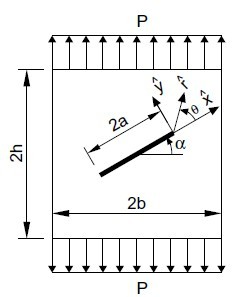
\includegraphics{chapter1/img/crackproblem.jpg}}
    % \end{figure}
    % /* cspell:enabled*/

%!TEX root = ../thesis.tex

\chapter{Literature review}

\section{Overview of numerical methods}

    \subsection{Finite element method}

    \subsection{Boundary element method}

    \subsection{Isogeometric analysis}

\section{Scaled boundary finite element method}

\section{Approaches for meshing automation}

    \subsection{Initial Graphics Exchange Specification (IGES) file}

    \subsection{Non-Uniform Rational B-Spline (NURBS)}

\section{Conclusions}

\chapter{Isogeometric enhanced SBFEM in 2D}
    %!TEX root = ../thesis.tex
\section{Background}
% 1.	Structural analysis and design: history and what is desired for.
\paragraph{}
Structural engineering is one of the aspects in civil engineering that aims at the design of the structure which supports the loads without failure.
The loads imposed may be any physical forces due to gravity, wind action, vibration, temperature change, etc.
In the ancient age, it helped the people to build and maintain mega-structure such as pyramid and sphinx in Egypt.
Nowadays, thanks to the tremendous development in mathematics and material science, an increasingly wider range of different complex structures becomes possible to analysis.

% 2.	Computer aided-design and its application in structural engineering and others
\paragraph{}
As a result of the increasingly complicated geometry in structural engineering and the birth of the computer, Computer Aided Design (CAD) has been developed in 1980s \citep{Dav2008}.
The first Unigraphics System (for 2D modelling and drafting) was sold by United Computing in 1975 \citep{Ste2010}.
Nowadays, CAD has been widespread and won significant popularity.
A predominant amount of the designs delivered to structural engineers are generated by the help of commercial CAD softwares.
Besides, the CAD has also been extended to other fields especially mechanical and aerospace engineering where extreme complex geometry are treated.

% 3.	Finite element method (this needs to be expanded) and other numerical method (meshless, XFEM, particle based methods, etc.
\paragraph{}
The traditional structural analysis method which depends on a closed form mathematical solution becomes incapable to handle the highly complicated geometric input.
This motivated the Finite element method (FEM) which constitutes a general tool for the numerical solution of partial differential equations in engineering and applied science to be proposed \citep{Ucb2010}.
It did not achieve enormous popularity until early 1950s, when digital computer was developed.
After that, the method was refined with the help of variational methods from Lord Rayleigh (1870) and W. Ritz (1909) as well as the Galerkin's weighted-residual approach \citep{Fel1994}.
Then, great amount of research has been conducted on the FEM in terms of mathematics and applications, contributing to its dominance over numerical method in solid mechanics and structural analysis by the beginning of the 1990s \citep{Clo1980}.
Although it is a principle method for solving complex problems in the engineering field, lack of the local mesh refinement and the inability to formulate unbounded domain restrict the usage of the FEM in some area.
As a consequence, other numerical methods such as Boundary Element Method (BEM) \citep{Li2011,WARDLE1984525} and the Extended FEM (X-FEM) \citep{Moes1999} were proposed.
In BEM, only the boundary was discretised, contributing to a reduction of the spatial dimension by one.
Besides, the problem involves the unbounded domain can be solved naturally.
Nevertheless, the fundamental solution satisfying the governing differential equations in the domain must be available.
Unfortunately, this fundamental solution may be extremely complex.
The X-FEM extended the FEM to solve problems with localized features that are not efficiently resolved by mesh refinement.
Compared to the traditional FEM, the X-FEM exhibits a strong ability of modeling the fractures in the material.

% 4.	Finite element mesh generation and meshing burden (say Yan’s paper on mesh generation and Albert’s thesis)
\paragraph{}
The FEM could be one of the most popular numerical methods in engineering analysis.
In the FEM, a meshing procedure that discretize the problem domain into individual elementary components or ``elements'' is necessary.
The solution of the whole system is calculated by assembling its discretized elements.
However, creation of mesh in FEM can be expensive in terms of time and human resource.
Numerous studies have been conducted for an automatic mesh generation algorithm \citep{owen2000,Blacker1993,doi:10.1002/fld.1650081003,doi:10.1093/comjnl/24.2.167}.

% 5.	Adaptive finite element analysis
\paragraph{}
When complex geometric input is involved, chances are that a considerably fine mesh is required to capture the localized phenomena.
However, a naive implemented mesh generation algorithm usually produce a uniform mesh where small elements are created even though they are only necessary in limited areas.
Hence the adaptive finite element analysis was proposed to maximize the quality of the numerical solution for a given amount of the computational effort.
In this method, tiny elements are generated at the required areas only and coarse mesh is expected for the rest.
Since the stress or the displacement is unknown before the numerical method is conducted, an adaptive mesh can be difficult to be generated based on the geometry and boundary condition only.
As a consequence, the concept of the ``posteriori error estimator'' was introduced to estimate the error contribution of each element based on the solution calculated from the FEM \citep{Duval2018, doi:10.1002/gamm.201490020,PRUDHOMME20091887,BAUMAN2009799}.

% 6.	Isogeometric analysis
\paragraph{}
In the existing computational methods, the geometry is interpolated by high order polynomials and the exact geometry is neglected due to its intricacy.
However, the accuracy of adopting it into computational mechanics seems to be limited \citep{Sza2004}.
Tensor product Non-Uniform Rational B-spline (NURBS) is a well-known curve and surface representation method and has been adopted as a standard in computer graphics, computer-aided-design (CAD) \citep{Nas2003} and Initial Graphics Exchange Specification (IGES) since 1983 \citep{IGES1983}.
Nowadays, the employment of rational polynomial functions in description of geometry in CAD/CAM applications is becoming more and more extensive \citep{Pie1987} and the CAD has been widespread and won even more popularity than the FEM does.
While, the geometric descriptions adopted by engineers today for CAD and that for analysis are totally different.
Furthermore, frequent design modifications in fast pace, modern society restricts the usage of analysis if a new mesh cannot be created in a short duration.
\paragraph{}
Creation of mesh in FEM can be expensive in terms of time and human resource.
One possible solution is trying to replace the geometric modelling tool in FEM by something more CAD-like.
NURBS, for example, is a standard mathematical model utilized in CAD industry.
Exact CAD geometric boundary is achieved with the help of the NURBS curve and surface.
This idea to be geometrically exact with a minimum discretization was adopted in Isogeometric analysis developed in 2005 \citep{Hug2005b} and further refined recently \citep{Zhang2007,Hug2005b,Cot2006,Cot2009,Baz2006a,Baz2006b}.
Furthermore, a simplified mesh refinement method by omitting the necessity for communication with the CAD geometry once the initial shape was received is also targeted \citep{Cot2007}.
It shows advantage in the structure analysis, fluid mechanics \citep{Buf2011} and dynamics \citep{Cot2006}.

% 7.	Scaled boundary finite element method
\paragraph{}
A Scaled Boundary finite element method (SBFEM) which has similarity with both the FEM and the BEM is proposed to eradicate the necessity of fundamental solution in BEM.
SBFEM is a novel semi-analytical approach developed by Wolf and Song \citep{Wol1999}.
As a method developed based on the FEM and the BEM, the SBFEM is a fundamental-solution-less boundary element method which keeps the benefits of the both as well as provides some effective solutions to the limitations to the FEM and the BEM \citep{Wol1999}.
The fundamental solution is no longer required, spatial dimension is reduced by one as only the boundary is meshed with surface elements which leads to a decline in the number of unknowns and achievement of infinite boundary \citep{Wol2003}.

%  ------------------------------------------- %

\section{State of the problem}
\label{intro_sec:problem}
\paragraph{}
In current Isogeometric analysis, accuracy problems with numerical integration of a rational polynomials attract significant attention \citep{Hug2010,Sev2011,Aur2012}.
Furthermore, incapability to create a set of control points to fit an inhomogeneous essential boundary condition may lead to considerable errors and lower converge speed due to the non-interpolatory characteristics of the NURBS \citep{Wang2010,Wol2011,Koo2013}.
Besides, although numerous amount of research has been conducted on improving the algorithm efficiency \citep{Boo1972,Qin1996,Cho1990,Gra1992,Pan2001,Wang2012}, most of the time is devoted to calculate the basis function which restricts the usage of high order basis function in 3D problems.
Moreover, one of the most critical problems in the existing Isogeometric analysis lies in the dimension incompatibility.
It is based on FEM where 3D NURBS solids are required for meshing in 3D problems but only the boundary is described in CAD system.
Further meshing process for converting input surface data to higher dimension physical geometry in isogeometric analysis has been referred to as ``analysis-aware modelling'' \citep{Coh2010}.
Considerable research on solving this incompatibility by domain parameterization has been performed using a variety of methods \citep{Yang2007,Aig2009,Mar2009,Qian2011}.

% mesh generation
\paragraph{}
the conventional FEM allows only hexahedron, tetrahedron, wedge and pyramid in 3D and triangular and quadrilateral elements in 2D which poses a heavy burden on mesh generation.
In order to achieve a reasonably accurate result, the mesh of the traditional FEM is required to conform to the boundary of the problem domain.
One rough estimate provided by \cite{Hug2005} suggests that more than half of the overall analysis time is spent on meshing in the industries such as automotive and aerospace where complex shapes are involved.
As a consequence, it could be necessary to develop an automatic mesh generation algorithm using limited types of shapes \citep{Frey:2007:MGA:1205626}.

% adaptive mesh refinement
\paragraph{}
Numerous research has been conducted on the ``posteriori error estimator'' to achieve an adaptive analysis and it has been developed in the FEM \citep{doi:10.1002/nme.1620330702,doi:10.1002/nme.1620330703, BOROOMAND1999127, ZIENKIEWICZ1999111, Ainsworth1993}, the BEM \citep{Zhao1998, Guiggiani1990, KAMIYA1992223} and the SBFEM \citep{NME:NME439}.
However, some of these error estimators require extra works such as stress recovery.
Besides, it could be difficult to determine the most suitable error indicator to a given problem.
Furthermore, the threshold is taken manually which limits the usage of several indicators as the number of the threshold grows quadratically as the number of the estimators increases.



%  ------------------------------------------- %
\section{Objective and significance}
\paragraph{}
As discussed in Sec.~\ref{intro_sec:problem}, there are several limitations associated with the existing numerical methods.
This thesis aims at developing a complete and systematic numerical method where all procedures are conducted without human involvement for an arbitrary geometric input in both 2D and 3D situations.
After the design files (IGES file and STL file in 3D) are delivered in electronic form, the proposed method shall be able to parse the geometric input, generate the mesh (quadtree in 2D and octree in 3D), determine the result using SBFEM and refine the mesh based on the error estimator automatically.
The SBFEM is adopted as it requires only the boundary information and hence provides a seamless integration with the CAD modeling.
The main objectives of this thesis are as follows
\begin{enumerate}
    \item Minimize human effort spent on structural analysis
    \item Be compatible with arbitrary geometric input in both 2D and 3D
    \item Generate high quality mesh
    \item Retain exact geometry
    \item Develop a robust, extensible and flexible error estimator
\end{enumerate}
Accomplishing tasks mentioned above makes significant contributions to solve the practical engineering problems automatically.
Furthermore, a new error estimator trained using machine learning algorithm allows unlimited number of indicators to be used.

%  ------------------------------------------- %
\section{Outline of the thesis}
\paragraph{}
In the next chapter, a literature review on the existing numerical methods including the Isogeometric analysis and the SBFEM, the automatic mesh generation algorithm and the adaptive mesh refinement is presented.
The advantages and disadvantages of different methods are critically discussed.

\paragraph{}
In Chapter 3, the idea of the isogeometric analysis is extended to the SBFEM to solve 2D problem including linear elasticity and linear elastic fracture mechanics.
The NURBS basis functions are adopted as the shape functions in the SBFEM instead of the conventional Legendre polynomials.
Some key formulations in linear elasticity and linear elastic fracture mechanics in the SBFEM using the NURBS shape functions are derived.
In order to perform a numerical integration on piecewise polynomials, a knot insertion is adopted to convert a piecewise polynomial to multiple non-piecewise polynomials.
NURBS curve fitting is also introduced to enforce the stress boundary condition.

\paragraph{}
Chapter 4 implements an IGES adaptor which can convert the geometric information stored in IGES file into polylines.
A quad-tree based mesh generation algorithm is developed to handle arbitrary geometric input from these polylines.
In order to retain the exact geometry, the intersection point on the polyline is projected back onto the original NURBS curve.
The projection is accelerated using the convex hull property and the quick hull algorithm is hence introduced.
Hard point treatment is developed in order to handle the multiple material interfaces, sharp edges or cracks.
Optimization algorithms such as bucket sort are adopted to improve the computational efficiency of the mesh generation.
Stress analysis is conducted on 2D linear elasticity problems.

\paragraph{}
In Chapter 5, an adaptive mesh refinement algorithm is proposed by the help of machine learning.
Expressions related to the eigenvalues of the SBFEM formulation together with some key geometric properties of the scaled boundary finite element are obtained as the error indicators.
The models trained by the Multilayer Perceptron (MLP), the Support Vector Machine (SVM) using radial kernel function and the random forest are compared and the MLP model which achieves the best performance is used.
In order to improve the accuracy of the MLP, regularization methods including bagging and dropout are adopted.
Due to the lack of eigenvalue error indicator in first order triangular element, method that eliminates these situation is produced.
A matrix representation of NURBS curves is presented to achieve a higher efficiency and stability in calculating the intersections between a line and a NURBS curve.
Stress analysis is conducted on 2D linear elasticity problems.

\paragraph{}
Chapter 6 references an octree based automatic mesh generation algorithm based on the STL file in 3D \citep{Liu2017}.
In order to retain the exact geometry, a method that can project intersection points on the triangular surfaces back to their origin NURBS surfaces is developed.
Another method that can calculate the intersection point between an edge in the scaled boundary finite element and the NURBS surface is also presented for the purpose of exact geometry.
The matrix representation of the NURBS surface in 3D is introduced to improve the computational efficiency and stability of the calculation of the intersection.
Splitting NURBS surfaces is adopted to accelerate the algorithm in both point projection and intersection calculation.
The computational efficiency of them are further improved by utilizing the strong hull properties of the NURBS surface and hence the quick hull algorithm in 3D is introduced.

\paragraph{}
Chapter 7 presents conclusions to the research.
Possible future works are proposed.

%!TEX root = ../thesis.tex

\chapter{Quad-tree mesh and auto refinement in 2D analysis based on error}

\section{Introduction}

\section{CAD output in 2D}

\section{NURBS utilization}

    \subsection{Distance function}

    \subsection{Finding intersections}

    \subsection{Optimization}

\section{Quad-tree structure}

\section{Conclusions}
%!TEX root = ../thesis.tex

\chapter{Adaptivity}

\section{Introduction}

\section{Lambda error indicator in SBFEM}

\section{Artificial neural network}

    \subsection{Learning algorithms}

    \subsection{Optimization algorithms}

        \subsubsection{Quasi-Newton methods}

        \subsubsection{Stochastic gradient descent}

        \subsubsection{Stochastic gradient-based optimizer proposed by Kingma, Diederik, and Jimmy Ba}

    \subsection{Activation function}

        \subsubsection{Identity}

        \subsubsection{Logistic}

        \subsubsection{Tanh}

        \subsubsection{Rectified linear unit function}

    \subsection{Learning rate}

    \subsection{Backpropagation algorithm}

\section{Multi-layer perceptron}

\section{Conventional neural network(not decided yet)}

\section{Numerical examples}

\section{Conclusions}


%!TEX root = ../thesis.tex

\chapter{Isogeometric enhanced SBFEM in 3D}

\section{Introduction}

\section{Formulation of SBFEM in 3D}

\section{CAD output in 3D}

\section{NURBS in 3D}

    \subsection{Surfaces division}

    \subsection{Finding projection}

    \subsection{Optimization using matrix representation}

\section{Numerical examples}

\section{Conclusions}
%!TEX root = ../thesis.tex

\chapter{Conclusions and recommendation}

% reference
\pagebreak
\bibliographystyle{plain}
\addcontentsline{toc}{chapter}{Bibliography}
\bibliography{ref}


\end{document}